\documentclass{./../div_teaching_slides}

\begin{document}
\title{ECON 340 \\ Economic Research Methods}
\author{Div Bhagia}
\date{Lecture 19 \\ Categorical Variables \& Interaction Terms}

%%%%%%%%%%%% 
\begin{frame}[noframenumbering, plain]
\maketitle
\end{frame}


%%%%%%%%%%%%
\begin{frame}{Fitting a Line}
Linear relationship (with some error):
$$ Y = \beta_0 + \beta_1 X + u  $$

Taking the conditional expectation:
$$ E(Y | X) =  \beta_0 + \beta_1 X + E(u | X)  $$

With $E(u | X)=0$, 
$$ E(Y | X) =  \beta_0 + \beta_1 X   $$

OLS fits a linear line between average $Y$ at each $X$ and $X$. 
\end{frame}

%%%%%%%%%%%%
\begin{frame}{Hypothetical Data: $E(wages|educ)$ and $educ$}
\centering
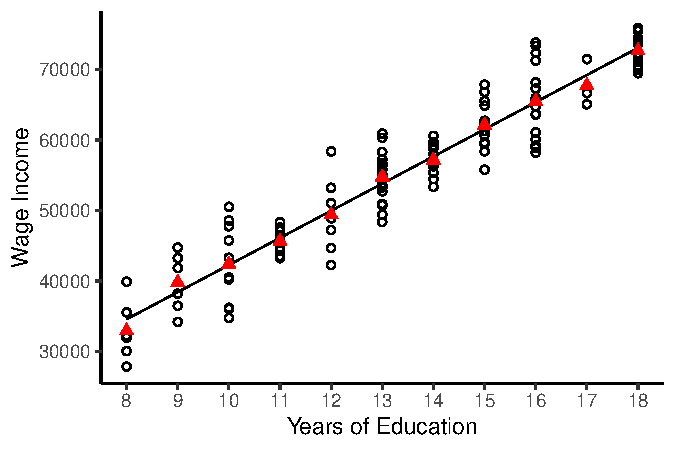
\includegraphics{./../../output/lrm_mean_fit.pdf}
\end{frame}

%%%%%%%%%%%%
\begin{frame}{Dummy Variables}
What if the independent variable is a binary variable that takes two values 1 and 0?  
$$ Y = \beta_0 + \beta_1 D + u  $$ \\~\\
Taking conditional expectation (assuming exogeneity):
\begin{align*}
	E[Y | D=1] &= \beta_0 + \beta_1 \cdot 1  = \beta_0 + \red{\beta_1} \\
	E[Y | D=0] &= \beta_0 + \beta_1 \cdot 0 = \beta_0 
\end{align*}
So, $$\red{\beta_1} = E[Y | D=1]-E[Y | D=0] $$  
\end{frame}

%%%%%%%%%%%%
\begin{frame}{ACS Data: Gender Wage Gap}
\centering  \small \vspace{1.25em}

% Table created by stargazer v.5.2.3 by Marek Hlavac, Social Policy Institute. E-mail: marek.hlavac at gmail.com
% Date and time: Thu, Nov 02, 2023 - 11:46:49
\begin{tabular}{@{\extracolsep{5pt}}lc} 
\\[-1.8ex]\hline 
\hline \\[-1.8ex] 
\\[-1.8ex] & Wages \\ 
\hline \\[-1.8ex] 
 Intercept & 67,220.17$^{***}$ \\ 
  & (439.87) \\ 
  & \\ 
 Female & $-$14,661.12$^{***}$ \\ 
  & (637.27) \\ 
  & \\ 
\hline \\[-1.8ex] 
Observations & 17,578 \\ 
R$^{2}$ & 0.03 \\ 
\hline 
\hline \\[-1.8ex] 
\textit{Note:}  & \multicolumn{1}{r}{$^{*}$p$<$0.1; $^{**}$p$<$0.05; $^{***}$p$<$0.01} \\ 
\end{tabular} 
 \\ \vspace{1.5em}
\end{frame}

%%%%%%%%%%%%
\begin{frame}{Dummy Variables: Interpretation}
As before, to interpret $\beta_1$ as the causal impact of gender on wages, we need: $$E(u|female)=0$$ \\~\\
Meaning that omitted factors that impact wages are uncorrelated with gender, which implies:
$$\beta_1 = E[wages | female=1]-E[wages | female=0] $$ \\~\\

However, even if exogeneity doesn't hold, $\hat{\beta}_1$ still captures the difference in average wages of men and women in our sample.  
\end{frame}


%%%%%%%%%%%%
\begin{frame}{Dummy Variables in Multiple Regression}
$$ Wages = \beta_0 + \beta_1 Age + \beta_2 Female +  u  $$ \\~\\
Taking conditional expectation (assuming exogeneity):
\begin{align*}
	E[Wages | Age, Female=1] &= (\beta_0+\red{\beta_2}) + \beta_1 Age
 \\
	E[Wages | Age, Female=0] &= \beta_0 + \beta_1 Age
	\end{align*} \\~\\
\end{frame}

%%%%%%%%%%%%
\begin{frame}{ACS Data: Wages and Age}
\centering  \small 
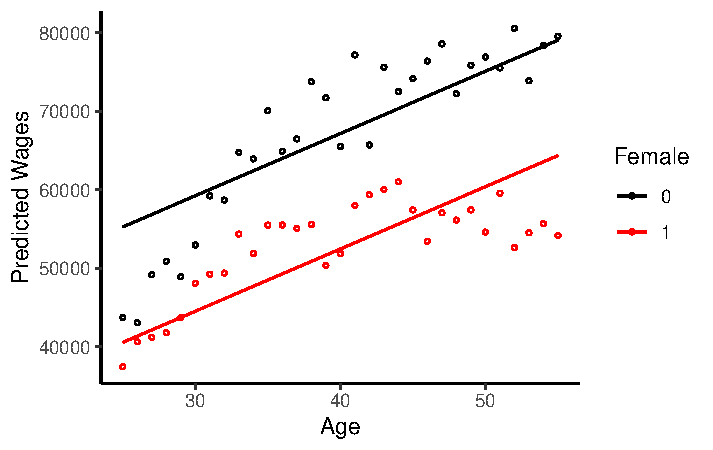
\includegraphics{./../../output/fit_gender_age.pdf} \\ \vspace{1.5em}
\end{frame}

%%%%%%%%%%%%
\begin{frame}{Interaction Terms}
We can also include interaction terms in our model as follows:
$$ Wages = \beta_0 + \beta_1 Age + \beta_2 Female + \beta_3 Female \times Age +  u  $$ \\~\\
Taking conditional expectation (assuming exogeneity):
\begin{align*}
	E[Wages | Age, Female=1] &= (\beta_0+\red{\beta_2}) + (\beta_1+\red{\beta_3}) Age
 \\
	E[Wages | Age, Female=0] &= \beta_0 + \beta_1 Age
	\end{align*} \\~\\
Now the impact of $X$ on $Y$ varies with $D$.
\end{frame}

%%%%%%%%%%%%
\begin{frame}{ACS Data: Wages and Age}
\centering
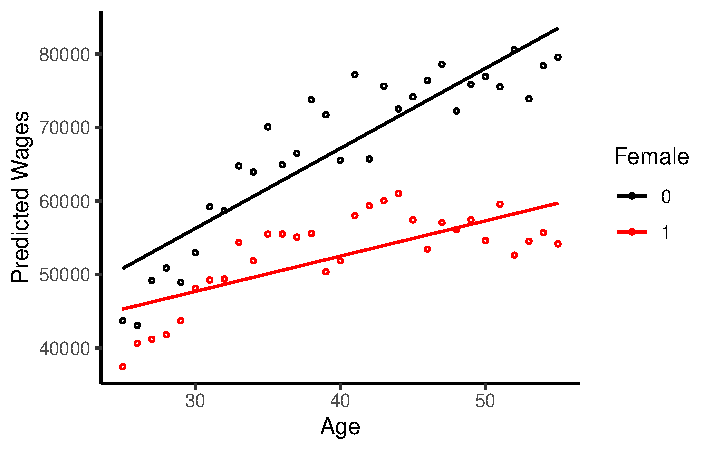
\includegraphics{./../../output/fit_gender_age_inter.pdf}
\end{frame}

%%%%%%%%%%%%
\begin{frame}{Interaction of Two Dummy Variables}
\vspace{-1em}
$$ wages = \beta_0 + \beta_1 Female + \beta_2 Hispanic + \beta_3 Female \times Hispanic +  u  $$ \\~\\
Average wages for Non-Hispanic Males:
$$ E(wages|Hispanic=0, Female=0) = \beta_0  $$ 
Average wages for Non-Hispanic Females:
$$ E(wages|Hispanic=0, Female=1) = \beta_0 + \red{\beta_1}  $$
\end{frame}

%%%%%%%%%%%%
\begin{frame}{Interaction of Two Dummy Variables}
\vspace{-1em}
$$ wages = \beta_0 + \beta_1 Female + \beta_2 Hispanic + \beta_3 Female \times Hispanic +  u  $$ \\~\\
Average wages for Hispanic Males:
$$ E(wages|Hispanic=1, Female=0) = \beta_0 + \beta_2  $$ 
Average wages for Hispanic Females:
$$ E(wages|Hispanic=1, Female=1) = \beta_0 + \red{\beta_1} + \beta_2 + \red{\beta_3}  $$
\end{frame}

%%%%%%%%%%%%
\begin{frame}{ACS Data: Gender and Ethnicity}
\vspace{-0.1em}
\centering  \small  

% Table created by stargazer v.5.2.3 by Marek Hlavac, Social Policy Institute. E-mail: marek.hlavac at gmail.com
% Date and time: Tue, Apr 18, 2023 - 18:20:28
\begin{tabular}{@{\extracolsep{5pt}}lc} 
\\[-1.8ex]\hline 
\hline \\[-1.8ex] 
\\[-1.8ex] & Wages \\ 
\hline \\[-1.8ex] 
 Intercept & 70,179.09$^{***}$ \\ 
  & (473.52) \\ 
  & \\ 
 Female & $-$16,046.81$^{***}$ \\ 
  & (683.42) \\ 
  & \\ 
 Hispanic & $-$19,367.71$^{***}$ \\ 
  & (1,211.46) \\ 
  & \\ 
 Female X Hispanic & 8,163.75$^{***}$ \\ 
  & (1,788.04) \\ 
  & \\ 
\hline \\[-1.8ex] 
Observations & 17,578 \\ 
R$^{2}$ & 0.05 \\ 
\hline 
\hline \\[-1.8ex] 
\textit{Note:}  & \multicolumn{1}{r}{$^{*}$p$<$0.1; $^{**}$p$<$0.05; $^{***}$p$<$0.01} \\ 
\end{tabular} 
 \\ \vspace{1.5em}
\end{frame}

%%%%%%%%%%%%
\begin{frame}{Variable with Multiple Categories}
	Five education categories:
	 $$ \{\text{Less than HS, HS Grad, Some College, College Degree, >College} \} $$ \\~\\
	 Add four dummy variables to the regression (why not five?):
	 $$ wages = \beta_0 + \beta_1 HS + \beta_2 SomeCol + \beta_3 Col + \beta_4 MoreThanCol +  u  $$ \\~\\
	 Reference category: Less than HS \\~\\
	 Coefficients capture the difference between average wages for that category and average wages for \textit{less than HS}. 
\end{frame}

%%%%%%%%%%%%
\begin{frame}{Variable with Multiple Categories}
\centering \vspace{1em}

% Table created by stargazer v.5.2.3 by Marek Hlavac, Social Policy Institute. E-mail: marek.hlavac at gmail.com
% Date and time: Tue, Apr 18, 2023 - 18:20:27
\begin{tabular}{@{\extracolsep{5pt}} cc} 
\\[-1.8ex]\hline 
\hline \\[-1.8ex] 
Education & Wages \\ 
\hline \\[-1.8ex] 
Less than HS & 36090.83 \\ 
High School & 44546.88 \\ 
Some College & 50182.94 \\ 
College Degree & 71527.75 \\ 
More than College & 87775.73 \\ 
\hline \\[-1.8ex] 
\end{tabular} 

\end{frame}

%%%%%%%%%%%%
\begin{frame}{Variable with Multiple Categories}
\centering \vspace{-0.5em} \footnotesize

% Table created by stargazer v.5.2.3 by Marek Hlavac, Social Policy Institute. E-mail: marek.hlavac at gmail.com
% Date and time: Tue, Apr 18, 2023 - 18:23:01
\begin{tabular}{@{\extracolsep{5pt}}lc} 
\\[-1.8ex]\hline 
\hline \\[-1.8ex] 
\\[-1.8ex] & Wages \\ 
\hline \\[-1.8ex] 
 Intercept & 36,090.83$^{***}$ \\ 
  & (1,386.07) \\ 
  & \\ 
 High School & 8,456.05$^{***}$ \\ 
  & (1,496.75) \\ 
  & \\ 
 Some College & 14,092.11$^{***}$ \\ 
  & (1,515.36) \\ 
  & \\ 
 College Degree & 35,436.92$^{***}$ \\ 
  & (1,499.47) \\ 
  & \\ 
 More than College & 51,684.90$^{***}$ \\ 
  & (1,559.17) \\ 
  & \\ 
\hline \\[-1.8ex] 
Observations & 17,578 \\ 
R$^{2}$ & 0.15 \\ 
\hline 
\hline \\[-1.8ex] 
\textit{Note:}  & \multicolumn{1}{r}{$^{*}$p$<$0.1; $^{**}$p$<$0.05; $^{***}$p$<$0.01} \\ 
\end{tabular} 

\end{frame}

%%%%%%%%%%%%
\begin{frame}{Binary Dependent Variable}
What if we have a binary variable on the left-hand side?

$$ emp = \beta_0 + \beta_1 educ  + u  $$

$$ E[emp|educ] = \beta_0 + \beta_1 educ    $$

Note that, 
$$ E[emp|educ] = P(emp=1|educ) = \beta_0 + \beta_1 educ $$ 

So, $\beta_1$ can be interpreted as the change in the probability of being employed. This is called the Linear Probability Model.
\end{frame}

%%%%%%%%%%%%%%%%%%%%
\begin{frame}{What's next?}
\begin{witemize}
  \item Next week, on Tuesday (11/07), we will continue with the linear regression model
  \item \textbf{No class on Thursday} (11/09) as I am traveling for a conference. Use this time to review the linear regression model and work on Problem Set 4.
  \item Problem Set 4 is due on the following Tuesday (11/14)
  \item The week after next, we will learn to conduct regression analysis in R before going into the fall break. 
\end{witemize}
\end{frame}



\end{document}